\documentclass[12pt]{article}
\usepackage[utf8]{inputenc}
\usepackage{amsmath}
\usepackage{multicol}
\usepackage{multirow}
\usepackage{listings}
\lstset{
    breaklines=true,
    breakatwhitespace=true
}
\usepackage{graphicx}
\usepackage[table, svgnames, dvipsnames]{xcolor}
\usepackage{longtable}
\usepackage[hidelinks]{hyperref}
\usepackage{makecell, cellspace, caption}
\usepackage{enumitem}
\usepackage{geometry}
\usepackage{titling}

\renewcommand{\contentsname}{Indice}

\title{
  
\includegraphics[height=0.20\textheight]{images/logo.png}\\
  \vspace{1cm}
  \materia\\
  \projectName
}
\author{Giuseppe Napoli - 1000012802}
\date{A.A. 2024/25}

% Variabili personalizzate
\newcommand{\materia}{Intelligenza Artificiale e Laboratorio}
\newcommand{\projectName}{Vertex Cover Solver}
\newcommand{\docenteUno}{Prof. Vincenzo Cutello}
\newcommand{\docenteDue}{Prof. Mario Francesco Pavone}

% Definizione del frontespizio
\pretitle{
  \begin{center}
      \LARGE
      \line(1,0){300}\\
      \vspace{0.5cm}
      \bfseries
    }
    \posttitle{
      \line(1,0){300}\\
      \vspace{1cm}
  \end{center}
}

\begin{document}

\maketitle

\section*{Docenti}
\begin{itemize}
  \item \docenteUno
  \item \docenteDue
\end{itemize}

\newpage
\tableofcontents
\newpage
\section{Introduzione}

Il \emph{Vertex Cover} è un problema classico della teoria dei grafi e dell’ottimizzazione combinatoria, in cui si cerca un insieme di vertici tale da \emph{coprire} (o intercettare) tutti gli archi di un grafo. Nella sua variante pesata (\emph{Weighted Vertex Cover}), ad ogni vertice è associato un costo (o peso) e l’obiettivo consiste nel minimizzare la somma dei pesi dei vertici selezionati, garantendo al contempo la copertura di tutti gli archi. Questo problema risulta \emph{NP-hard}, rendendolo particolarmente sfidante dal punto di vista computazionale, soprattutto per istanze di grandi dimensioni.

Nel presente progetto, si è scelto di affrontare il Weighted Vertex Cover mediante una \emph{metaeuristica di tipo Tabu Search}, al fine di ottenere soluzioni di buona qualità in tempi ragionevoli, anche su istanze con dimensioni non trascurabili. La Tabu Search, introdotta da Fred Glover, è un approccio iterativo che combina una ricerca locale sistematica con una struttura di memoria (detta \emph{tabu}) in grado di gestire sia la cosiddetta \emph{short-term memory} (con lo scopo di evitare cicli o ritorni su soluzioni già visitate), sia la \emph{long-term memory} (orientata ad aumentare la diversificazione e l’esplorazione dello spazio delle soluzioni).

Nel prosieguo, verranno illustrate le principali caratteristiche dell’algoritmo, le scelte progettuali e implementative adottate --- con particolare attenzione ai parametri chiave (\emph{maxIterations}, \emph{tabuTenure} e \emph{maxNoImprovement}) --- e i risultati sperimentali ottenuti. Verranno infine discussi possibili sviluppi futuri e riflessioni personali emerse dal lavoro svolto.

\newpage
\section{Algoritmo}
\label{sec:Algoritmo}

\subsection{Panoramica Generale}

L'algoritmo adottato è una \textit{Tabu Search}, una metaeuristica che evita cicli memorizzando le mosse recenti in una \textit{tabu list}. Come descritto nell'Introduzione, il problema viene affrontato tramite una ricerca locale iterativa, partendo da una soluzione iniziale e modificandola per minimizzare il costo.

Ad ogni iterazione, vengono generate soluzioni vicine valutate tramite una funzione costo. La \textit{tabu list} impedisce di ripetere modifiche recenti per un numero prefissato di iterazioni, bilanciando esplorazione e ottimizzazione. Nei prossimi paragrafi verranno descritti i dettagli implementativi dell’algoritmo.

\subsection{Struttura Della Tabu Search}
\label{sec:TabuSearch}

L'algoritmo si basa su una ricerca locale iterativa, mantenendo una soluzione corrente e aggiornandola esplorando il vicinato. La qualità di ogni soluzione è valutata tramite una funzione costo, mentre una \textit{tabu list} impedisce il ripristino di mosse recenti, favorendo l'esplorazione di nuove configurazioni.

Gli elementi principali dell'algoritmo includono:
\begin{itemize}
    \item \textbf{Soluzione corrente}: insieme di vertici selezionati nel \textit{vertex cover}.
    \item \textbf{Migliore soluzione}: la configurazione con costo minimo trovata finora.
    \item \textbf{Tabu list}: insieme di mosse vietate per un numero limitato di iterazioni.
    \item \textbf{Vicinato}: soluzioni ottenute aggiungendo o rimuovendo vertici.
\end{itemize}

L'algoritmo prosegue fino al raggiungimento di un criterio di arresto, basato su un numero massimo di iterazioni o sull'assenza di miglioramenti per un intervallo predefinito. Il funzionamento dettagliato, inclusa la gestione della \textit{tabu list} e dei parametri principali (\texttt{tabuTenure}, \texttt{maxIterations}, \texttt{maxNoImprovement}), è illustrato nello pseudocodice della sezione successiva.

Tra i parametri fondamentali troviamo:
\begin{itemize}
    \item \textbf{\emph{maxIterations}:} numero massimo di iterazioni complessive.
    \item \textbf{\emph{tabuTenure}:} numero di iterazioni per cui una mossa rimane nella tabu list.
    \item \textbf{\emph{maxNoImprovement}:} numero massimo di iterazioni consecutive senza miglioramenti, oltre cui fermare l'algoritmo.
\end{itemize}

\subsection{Pseudocodice}

L'algoritmo segue un ciclo iterativo in cui si generano soluzioni vicine e si applicano criteri di selezione basati sulla \textit{tabu list} e sulla qualità della soluzione. La funzione di valutazione guida la ricerca, mentre i criteri di aspirazione permettono di ignorare vincoli tabu se si trova una soluzione migliore.

Il funzionamento è riassunto nel seguente pseudocodice:

\begin{lstlisting}[language=Python, caption=Pseudocodice della Tabu Search]
FUNCTION TABU_SEARCH(Graph, maxIter, tabuTenure, maxNoImprovement):
    bestSolution = INITIAL_SOLUTION(Graph)
    currentSolution = bestSolution.copy()
    tabuList = emptySet
    iterations = 0
    noImprovement = 0

    WHILE iterations < maxIter AND noImprovement < maxNoImprovement:
        neighbors = GENERATE_NEIGHBORS(currentSolution)
        bestNeighbor = SELECT_BEST(neighbors, tabuList, bestSolution)

        IF bestNeighbor is NULL:
            BREAK
        
        UPDATE_TABU_LIST(tabuList)
        tabuList.add(DETERMINE_MOVE(currentSolution, bestNeighbor), tabuTenure)
        
        currentSolution = bestNeighbor.copy()

        IF cost(currentSolution) < cost(bestSolution):
            bestSolution = currentSolution.copy()
            noImprovement = 0
        ELSE:
            noImprovement += 1

        iterations += 1

    RETURN bestSolution
\end{lstlisting}

Le principali operazioni sono:
\begin{itemize}
    \item \texttt{INITIAL\_SOLUTION}: genera una configurazione iniziale ammissibile.
    \item \texttt{GENERATE\_NEIGHBORS}: produce soluzioni vicine.
    \item \texttt{SELECT\_BEST}: sceglie la soluzione migliore rispettando le regole tabu.
    \item \texttt{UPDATE\_TABU\_LIST}: aggiorna la memoria tabu rimuovendo mosse scadute.
    \item \texttt{DETERMINE\_MOVE}: identifica la modifica necessaria per la transizione tra soluzioni.
\end{itemize}

L'algoritmo si arresta se il numero massimo di iterazioni è raggiunto o se non si verificano miglioramenti per un certo numero di iterazioni consecutive.

\subsection{Esecuzione e Parametri Principali}

In fase di esecuzione, l'algoritmo arresta la ricerca in presenza di due condizioni:
\begin{enumerate}
    \item Il \emph{numero totale di iterazioni} raggiunge \emph{maxIterations}.
    \item Non si osservano miglioramenti alla \emph{bestSolution} per più di \emph{maxNoImprovement} iterazioni consecutive.
\end{enumerate}

Le prestazioni (sia in termini di tempo di esecuzione che di qualità delle soluzioni) dipendono fortemente dalla scelta di parametri come \emph{maxIterations}, \emph{tabuTenure}, \emph{maxNoImprovement} e dalla definizione delle mosse nel \emph{vicinato}.

In questo lavoro, si è analizzato un range di valori per i parametri chiave (ad esempio, \emph{tabuTenure} variato tra 5 e 7, \emph{maxNoImprovement} tra 10 e 30), confrontando i risultati sia in termini di costi ottenuti sia di stabilità dell'algoritmo. I dettagli di tali sperimentazioni sono riportati nel Capitolo~\ref{sec:Risultati}.

% (Finisce il capitolo Algoritmo)

\newpage
\section{Scelte Progettuali}
\label{sec:ScelteProgettuali}

In questo capitolo vengono descritte e motivate le principali scelte progettuali e implementative che sono state adottate nello sviluppo dell'algoritmo di Tabu Search per il \emph{Weighted Vertex Cover}. Tali scelte riguardano sia la configurazione dei parametri, sia la modalità di gestione della memoria \emph{Tabu} (short-term e/o long-term), fino alle strategie di generazione del vicinato.

\subsection{Struttura della Soluzione e Gestione della Memoria Tabu}

La soluzione è rappresentata come un vettore binario di dimensione pari al numero di nodi del grafo, dove un valore "1" indica un nodo incluso nel \textit{vertex cover}, mentre "0" lo esclude. Il costo di una soluzione è dato dalla somma dei pesi dei nodi selezionati.

L'algoritmo utilizza una \textit{tabu list} per gestire la memoria a breve termine e prevenire cicli. Questa viene implementata come una mappa che associa ogni mossa proibita (es. aggiunta/rimozione di un nodo) a un contatore di scadenza. Ad ogni iterazione:
\begin{enumerate}
    \item Si decremetano i contatori delle mosse presenti nella \textit{tabu list}.
    \item Si rimuovono le mosse scadute.
    \item Si aggiunge la mossa appena effettuata con una durata pari a \texttt{tabuTenure}.
\end{enumerate}

I principali parametri di controllo dell'algoritmo sono:
\begin{itemize}
    \item \textbf{\texttt{maxIterations}}: numero massimo di iterazioni.
    \item \textbf{\texttt{tabuTenure}}: durata di una mossa nella \textit{tabu list}.
    \item \textbf{\texttt{maxNoImprovement}}: numero massimo di iterazioni senza miglioramenti prima di interrompere la ricerca.
\end{itemize}

Questa gestione consente all'algoritmo di evitare soluzioni già esplorate e favorire la diversificazione della ricerca. L'uso della memoria \textit{long-term}, basata sulla frequenza con cui un nodo è selezionato, è stato considerato ma non implementato in modo esteso.

\subsection{Generazione del Vicinato e Riflessioni sulle Scelte Progettuali}

Il vicinato è generato rimuovendo un nodo dal \textit{vertex cover}, purché la soluzione resti ammissibile, o aggiungendo un nodo se necessario per coprire archi scoperti. Si adotta un criterio \textit{strictly feasible}, evitando mosse che renderebbero la soluzione non valida. 

Questa strategia consente di mantenere soluzioni ammissibili e di esplorare lo spazio in modo controllato, evitando modifiche eccessivamente distruttive. La Tabu Search, grazie alla \textit{tabu list}, permette di bilanciare esplorazione e intensificazione della ricerca. 

Le scelte progettuali adottate si sono dimostrate efficaci nel garantire stabilità e qualità delle soluzioni, evitando minimi locali evidenti e mantenendo tempi di esecuzione contenuti anche su istanze di grandi dimensioni.

\subsection{Scelte di Implementazione e Linguaggio}

L'algoritmo è stato implementato in Java per sfruttare strutture dati efficienti e garantire buone prestazioni su istanze di grandi dimensioni. La \textit{tabu list} è gestita con una \texttt{HashMap<String, Integer>}, in cui la chiave rappresenta una mossa (es. \texttt{"REMOVE 5"}) e il valore indica il numero di iterazioni rimanenti prima della sua rimozione.

L'uso di un linguaggio compilato garantisce tempi di esecuzione più rapidi rispetto a linguaggi interpretati, riducendo l'overhead di gestione della memoria. La scelta di Java ha permesso inoltre una gestione semplice delle strutture dati e della modularità del codice.

% Fine capitolo

\newpage
\section{Risultati Sperimentali}
\label{sec:Risultati}

In questo capitolo vengono presentati e discussi i risultati ottenuti dall'implementazione dell'algoritmo \emph{Tabu Search} descritto nei capitoli precedenti. Per valutare il comportamento dell’algoritmo, si sono condotti test su diverse istanze del problema, variando i parametri chiave come \emph{tabuTenure}, \emph{maxNoImprovement} e la dimensione dei grafi.

\subsection{Setup Sperimentale}

Le prove sono state eseguite su una macchina con le seguenti specifiche:
\begin{itemize}
    \item \textbf{CPU:} Intel Core i7-1065G7 (1.30\,GHz)
    \item \textbf{RAM:} 16\,GB
    \item \textbf{Sistema Operativo:} WSL Ubuntu 20.04 (64 bit)
    \item \textbf{Linguaggio:} Java (OpenJDK 17)
\end{itemize}

Le istanze di test comprendono grafi con numero di nodi (\(n\)) variabile tra 20 e 800, e numero di archi (\(m\)) tra 60 e 10000. I pesi dei nodi sono interi positivi.

\subsection{Confronto tra Diverse Configurazioni di Parametri}

Per capire come i parametri influenzino le prestazioni, sono state confrontate diverse configurazioni di \emph{tabuTenure} (5, 7), \emph{maxNoImprovement} (10, 20, 30) e \emph{maxIterations} (500, 1000, 2000). In ciascun caso, l'algoritmo è stato eseguito 5 volte su ogni istanza, per ridurre la variabilità stocastica. A titolo di esempio, la tabella~\ref{tab:risultati1} riporta i risultati medi su un insieme di 3 istanze (piccola, media e grande).

\begin{table}[h!]
\centering
\caption{Risultati medi (5 run) per diverse configurazioni di \emph{maxIterations}, \emph{tabuTenure} e \emph{maxNoImprovement}.}
\label{tab:risultati1}
\begin{tabular}{l|c|c|c|c|c|c}
\hline
\textbf{Config.} & \textbf{n} & \textbf{m} & \textbf{maxIter.} & \textbf{tabuTenure} & \textbf{maxNoImpr.} & \textbf{Time (s)} \\
\hline
C1 & \multirow{6}{*}{20} & \multirow{6}{*}{60}  
& 500  & 5  & 10 & 0.0092 \\
C4 & &  & 500  & 7  & 20 & 0.0148 \\
C7 & & & 1000 & 5  & 20 & 0.0156 \\
C10 & & & 1000 & 10 & 30 & 0.021 \\
C13 & & & 2000 & 7  & 10 & 0.0134 \\
C16 & & & 2000 & 10 & 20 & 0.0168 \\
\hline
C2 & \multirow{6}{*}{100} & \multirow{6}{*}{500}  
& 500  & 5  & 10 & 0.0608 \\
C5 & & & 500  & 7  & 20 & 0.108 \\
C8 & & & 1000 & 5  & 20 & 0.0836 \\
C11 & & & 1000 & 10 & 30 & 0.0818 \\
C14 & & & 2000 & 7  & 10 & 0.062 \\
C17 & & & 2000 & 10 & 20 & 0.0926 \\
\hline
C3 & \multirow{6}{*}{800} & \multirow{6}{*}{10000}  
& 500  & 5  & 10 & 6.1008 \\
C6 & & & 500  & 7  & 20 & 6.7292 \\
C9 & & & 1000 & 5  & 20 & 6.7994 \\
C12 & & & 1000 & 10 & 30 & 7.2512 \\
C15 & & & 2000 & 7  & 10 & 6.856 \\
C18 & & & 2000 & 10 & 20 & 7.54 \\
\hline
\end{tabular}
\end{table}

\noindent
Dall’osservazione dei dati in tabella~\ref{tab:risultati1} emergono due punti essenziali:
\begin{itemize}
    \item \textbf{Dimensioni del grafo come fattore dominante:}
    passando da \((20,60)\) a \((800,10000)\) nodi/archi, si registra un salto netto dei tempi di esecuzione (dell’ordine di microsecondi-millisecondi a svariati secondi).

    \item \textbf{\emph{maxNoImprovement} come parametro più incisivo:}
    a parità di \emph{maxIterations} e \emph{tabuTenure}, valori minori di \emph{maxNoImprovement} (in particolare 10) mostrano i migliori tempi d’esecuzione, mentre configurazioni con \emph{maxNoImprovement} più alto fanno salire i tempi, seppur meno drasticamente del puro aumento di dimensione del grafo.
\end{itemize}

\subsection{Commenti sui Risultati}

Nel complesso, la Tabu Search così configurata è risultata:
\begin{itemize}
    \item \textbf{Affidabile}: produce soluzioni di buona qualità con bassa varianza fra diversi run.
    \item \textbf{Poco sensibile} ai parametri: variazioni dei parametri non cambiano in modo significativo i risultati, come visto in tabella~\ref{tab:risultati1}.
    \item \textbf{Scalabile} fino a grafi di alcune migliaia di archi, con tempi di esecuzione che rimangono in un range accettabile (alcuni secondi).
\end{itemize}

\begin{figure}[h!]
\centering
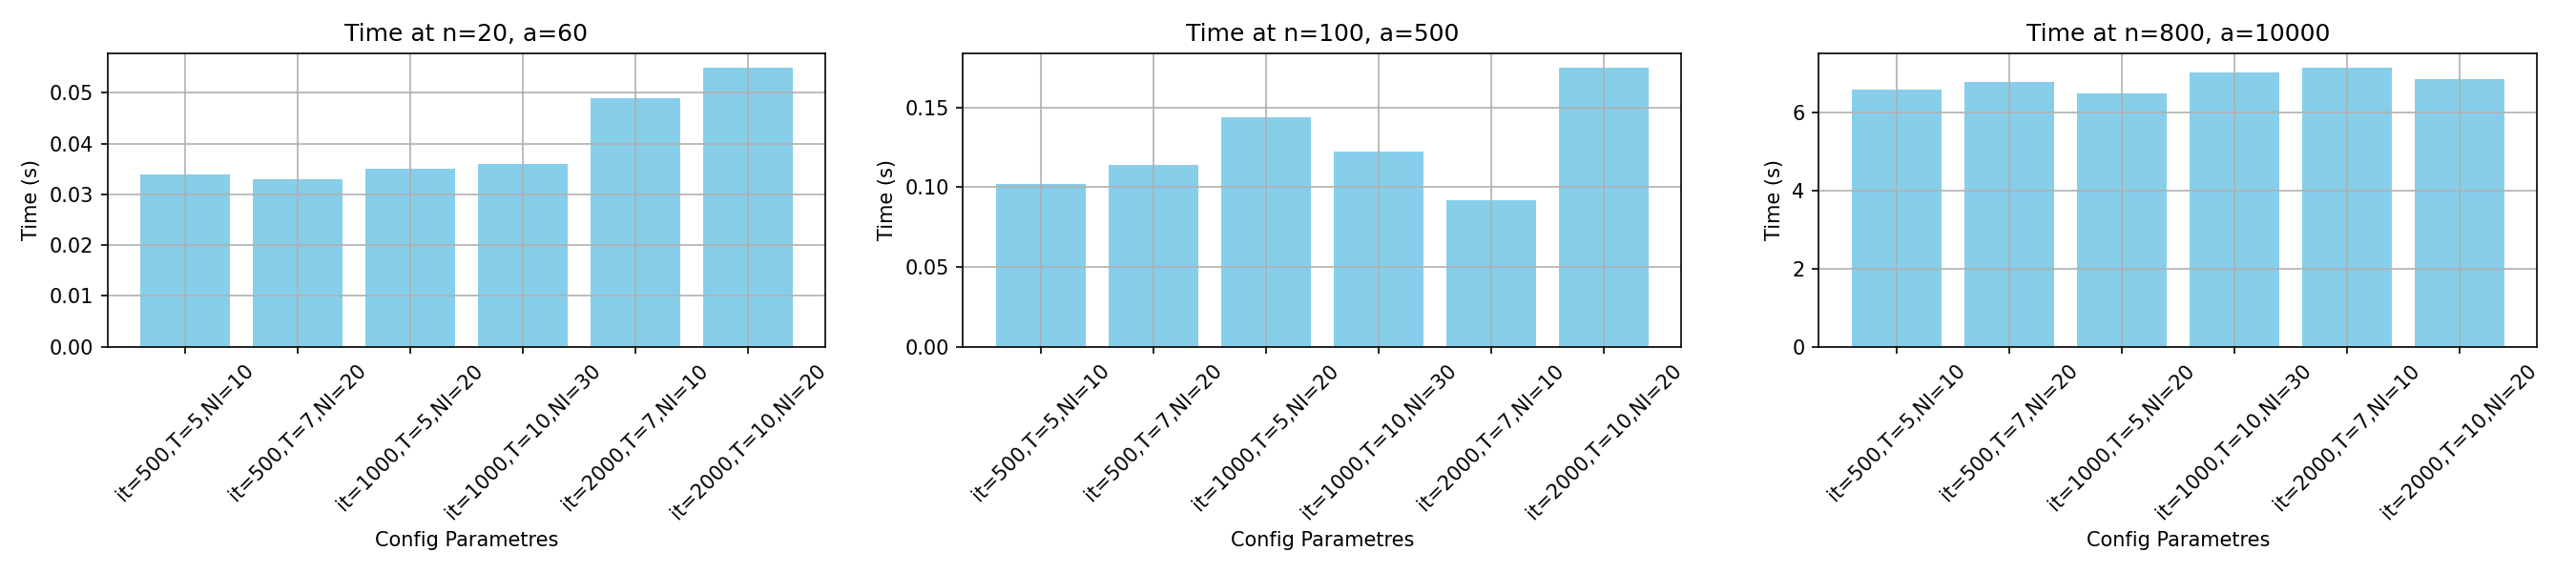
\includegraphics[width=1\textwidth]{images/scalability_plot.png} % Esempio di plot
\caption{Tempo di esecuzione medio in funzione della dimensione del grafo e della configurazione dei tre parametri.}
\label{fig:scalability}
\end{figure}

Una eventuale \emph{long-term memory}, basata sul conteggio di frequenza con cui i nodi appaiono o spariscono dal cover, potrebbe migliorare ulteriormente la diversificazione su istanze molto grandi, sebbene ciò comporti una maggiore complessità implementativa. Nel prossimo capitolo (\ref{sec:Conclusioni}) verranno esposti alcuni spunti di sviluppo e riflessioni conclusive sull'algoritmo e le sue prospettive future.

% Fine capitolo Risultati

\newpage
\section{Conclusioni}
\label{sec:Conclusioni}

Nel corso di questo progetto, è stato sviluppato un \emph{solver} per il problema del \emph{Weighted Vertex Cover} basato su una metaeuristica di tipo \emph{Tabu Search}. L’obiettivo principale era esplorare e applicare un approccio combinatorio in grado di trovare soluzioni di buona qualità in tempi computazionali ragionevoli, anche su istanze di dimensioni intermedie o relativamente grandi.

\subsection*{Riepilogo del Lavoro Svolto}
Il lavoro ha compreso:
\begin{enumerate}
    \item La definizione di una \emph{soluzione} come insieme di nodi (o vettore booleano) che copre tutti gli archi del grafo.
    \item L’implementazione di una \emph{Tabu Search}, con meccanismi di:
    \begin{itemize}
        \item \textbf{Short-term memory}, per evitare il ritorno immediato a soluzioni o mosse già visitate di recente.
        \item \textbf{Aspiration criterion}, che consente di ignorare lo stato \emph{tabu} se la soluzione candidata migliora la migliore soluzione globale.
    \end{itemize}
    \item L’analisi dei \emph{parametri} chiave dell’algoritmo (\emph{tabuTenure}, \emph{maxIterations}, \emph{maxNoImprovement}) e l’effetto della loro variazione sui risultati.
    \item Test sperimentali su istanze di diversa dimensione, con valutazione e confronto delle prestazioni (\emph{Best Cost} trovato, tempi medi, stabilità delle soluzioni).
\end{enumerate}

\subsection*{Valutazione delle Scelte Progettuali}
Le strategie adottate — in particolare la definizione del \emph{vicinato}, la gestione \emph{move-based} della Tabu List e il criterio di arresto basato su \emph{maxNoImprovement} — hanno dimostrato di produrre soluzioni di qualità. La Tabu Search, infatti, si è rivelata capace di evitare rapidamente i \emph{minimi locali} più ovvi e di diversificare sufficientemente la ricerca, specialmente quando si ottimizza il valore di \emph{tabuTenure}.

\subsection*{Sviluppi Futuri}
Tra le possibili estensioni o linee di lavoro future si possono evidenziare:
\begin{itemize}
    \item \textbf{Integrazione di una Long-term Memory}: per catturare le frequenze di aggiunta/rimozione di ciascun nodo e favorire una \emph{diversificazione} più ampia su istanze di grandi dimensioni.
    \item \textbf{Ibridazione con altre metaeuristiche}: ad esempio, un \emph{framework} che combini una fase di \emph{Genetic Algorithm} per generare popolazioni di soluzioni, seguita da un \emph{local search} Tabu Search per il refinement di ciascun individuo.
    \item \textbf{Parallelizzazione}: molte fasi della Tabu Search (generazione del vicinato, valutazione del costo) possono essere eseguite in parallelo, sfruttando architetture multicore o \emph{GPU}.
    \item \textbf{Benchmark su istanze molto grandi}: sarebbe interessante testare l’algoritmo su grafi con decine di migliaia di nodi e valutare le strategie di pruning o di riduzione del vicinato per abbattere i tempi di calcolo.
\end{itemize}

\subsection*{Considerazioni Finali}
Nel complesso, l’esperienza acquisita con questo progetto evidenzia la validità delle metaeuristiche come strumento efficace per problemi NP-hard. Nonostante la Tabu Search non garantisca l’ottimalità, le soluzioni ottenute risultano competitive rispetto ad approcci euristici più semplici, specialmente su istanze di dimensioni medio-grandi. Il lavoro svolto dimostra come la personalizzazione dei parametri e la cura della struttura \emph{tabu} siano fondamentali per ottenere le migliori prestazioni possibili, aprendo la strada a numerosi sviluppi futuri.

% Fine capitolo Conclusioni

\end{document}